\section{Exploration des interruptions en espace utilisateur.}
\label{sec:exploreUintr}

Pour cette partie, j'ai utilisé mes connaissances personnelles autour du système, du développement noyau, de Linux, ainsi que ce que j'ai appris en cours de \emph{programmation système}, de \emph{système d'exploitation}, d'\emph{architecture des ordinateurs} et \emph{Programmation des Architectures Parallèles}.

\subsection{Prérequis et accès}
\label{requirements}

Pour utiliser le mécanisme d'interruption en espace utilisateur, que nous allons abréger en \uintr{} dans la suite de ce document,
il est nécessaire d'avoir accès à un CPU \intel{} Sapphire Rapids.
Du fait qu'ils étaient sortis récemment, ils étaient assez difficiles d'accès.
\atos{} nous a donné accès, non sans difficulté, à une machine qui possède 2 CPU \intel{} Sapphire Rapids, lesquels sont des \intel{} Xeon\textsuperscript{\tiny{\textregistered}} Platinum 8470.
Les difficultés étaient liées à la disponibilité d'une machine, à trouver un endroit où l'installer et à s'assurer qu'elle soit connectée à un réseau accessible depuis l'Inria.
Nous avons donc obtenu un accès VPN qui utiliser l'ancien système VPN, car le nouveau ne fonctionnait pas.
Nous avons eu accès à la machine environ deux mois et demi après le début du stage.
La machine était déjà configurée avec le système d'exploitation Red Hat Enterprise Linux (RHEL) version 9.1 avec un noyau Linux version \emph{5.14.0-162.6.1}.
Elle possède également au moins une carte \emph{BXI} v2 que nous n'avons pas utilisées pendant le stage. % v2 == BXI 1.3

Il faut également avoir une version patchée du noyau Linux prenant en charge le nouveau mécanisme.
Cette version patchée n'est pas encore disponible dans la branche principale du noyau.
Cependant, elle est accessible sur le GitHub d'\intel{} \cite{intelUintrLinuxKernel}.
Elle est basée sur la version \emph{6.0.0}.
Nous avons donc téléchargé cette version patchée, puis nous l'avons compilée et installée sur la machine, toutes les commandes nécessaires pour cela sont disponibles en annexe.
Lors de la compilation, il est nécessaire d'activer le support des \uintr{} (Voir la figure \ref{fig:enableFeaturesInConfigMenu} en annexe).
Il est également possible d'activer le support permettant à un thread bloqué, c'est-à-dire non ordonnancé ou dans un appel système interruptible, de recevoir une \uintr{}.

Le mécanisme utilise de nouvelles instructions, donc une version récente du compilateur \emph{GCC} est nécessaire pour compiler les programmes utilisateurs qui utiliseront les \uintr{}.
Il faut donc la version \emph{11.3.0} ou plus récente de \emph{GCC}, et sur RHEL il faut la version \emph{12.1.1} ou supérieure.
Le support n'est pas encore disponible dans d'autres compilateurs comme \emph{LLVM-Clang} ou \emph{ICC}.
Pour compiler un programme utilisateur, il faut spécifier le flag de compilation \code{-muintr} pour les fichiers qui définissent un handler d'interruption ou qui utilisent les nouvelles instructions.

\subsection{Fonctionnement des interruptions en espace utilisateur}
\label{sec:uintr}

Dans le cadre de ce stage, nous avons étudié en détail le fonctionnement des interruptions ordinaires ainsi que le fonctionnement des interruptions en espace utilisateur.
Les \uintr{} n'était pas connus des équipes \emph{Inria} et \atos{}.

\subsubsection{Les interruptions}
\label{sec:interrupts}


Pour commencer, nous allons voire le fonctionnement des interruptions matérielles.
Nous nous concentrerons sur l'envoi d'interruptions entre deux processus fixés sur deux unités de calcul.
Pour ces interruptions les CPU disposent d'une unité dédiée à leur traitement, l'\emph{APIC} pour "Advanced Programmable Interrupt Controller".
Cette \emph{APIC} permet au système d'enregistrer un handler pour chaque interruption.
Le noyau définit un tableau appelé \emph{IDT} pour "Interrupt Descriptor Table" qui contient 256 entrées, correspondant à 256 interruptions possibles.
Les indices de l'\emph{IDT} sont des valeurs comprises entre 0 et 255, que l'on appelle également \textbf{vecteur}s d'interruption.
Parmi eux, les vecteurs entre 0 et 31 sont réservés pour les exceptions et les interruptions système,
les vecteurs entre 32 et 127 sont dédiés aux interruptions liées aux périphériques,
le vecteur 128 est réservé pour les appels système,
et les vecteurs entre 129 et 255 sont destinés à des utilisations diverses.

Il est important de savoir que chaque unité de calcul (processeur logique) possède un \emph{APIC ID} physique.
À titre informatif, le \emph{core ID} est un sous-ensemble de l'\emph{APIC ID}.

Pour déclencher une interruption, il y a quatre possibilités :

\begin{enumerate}
  \item Une exception déclenchée par un processeur (e.g. une division par zéro, un défaut de segmentation...).
  \item Une instruction comme \code{INT80 numSysCall} pour déclencher un appel système, ou bien \code{INT3} pour définir un point d'arrêt, ou encore \code{INTO}, \code{BOUND} et \code{INT n}.
  \item Des broches du CPU dédiées à la réception d'interruptions lancées à partir d'un périphérique.
  \item Demander à l'\emph{APIC} elle-même grâce à un registre \emph{ICR} pour "Interrupt Command Register".
  Il existe un \emph{ICR} par vecteur, donc il faut écrire l'\emph{APIC ID} du destinataire dans le \emph{ICR} du vecteur que l'on veut déclencher.
  Seul le CPU et le noyau peuvent modifier les \emph{ICR}. % TODO: est peut être les périphérique non ?
\end{enumerate}

On voit bien que les \emph{IRQ} fonctionnent au niveau du noyau et du CPU.

Nous allons voir un exemple d'envoi d'\emph{IRQ} entre deux unités de calcul en cours d'exécution.
Tout d'abord, l'initialisation des \emph{IRQ} se fait au démarrage du système et consiste principalement à définir les handlers noyau dans l'\emph{IDT}.
Il faut aussi définir quel vecteur nous voulons utiliser, le code du handler noyau qui sera invoqué,
comment l'utilisateur va contacter le système et comment faire l'identification du récepteur.
Pour cela, on peut appliquer un patch au noyau ou faire un module noyau.

Dans notre exemple, nous allons supposer que nous avons déjà patché le noyau en ajoutant des appels système et que nous avons choisi un vecteur.

Nous allons maintenant voir les étapes de l'envoi d'une \emph{IRQ}, illustrées sur la figure \ref{fig:sendInt} :

\begin{enumerate}[label=\protect\circled{\arabic*}]
  \item Le récepteur fait un appel système pour indiquer au noyau comment il veut être averti d'une interruption (e.g. un descripteur de fichiers qu'il va lire, un appel système bloquant, une zone mémoire où lire, un handler utilisateur, etc.).
  \item L'émetteur peut donc avertir le noyau qu'il faut envoyer une interruption.
  Pour cela, il peut utiliser un appel système ou écrire dans un descripteur de fichiers, par exemple.
  \item Le noyau détermine l'unité de calcul où se trouve le récepteur.
  Pour cela, il peut utiliser par exemple un \emph{PID} pour "Processus ID" donné par l'émetteur ou autre.
  Ainsi, il peut déterminer l'\emph{APIC ID} de l'unité de calcul à interrompre.
  \item Le noyau écrit donc l'\emph{APIC ID} dans le \emph{ICR} d'un vecteur déterminé à l'avance.
  L'émetteur reprend alors la main après un autre changement de contexte.
  \item L'\emph{APIC} va donc interrompre le récepteur qui va alors stopper son exécution et passer dans le noyau.
  Une fois dans le noyau, le handler va se déclencher et exécuter le code prévu au préalable (écriture dans un descripteur de fichiers, écriture dans une zone mémoire, déclenchement d'un handler utilisateur, etc.).
\end{enumerate}

\begin{figure}[H]
  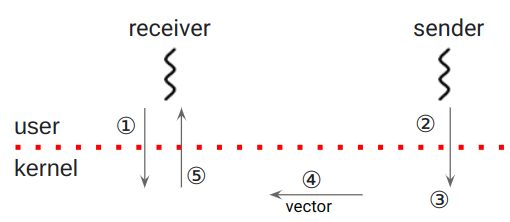
\includegraphics[width=\textwidth]{interruptSend}
  \caption{L'envoi d'une interruption ordinaire}
  \label{fig:sendInt}
\end{figure}

Lors du déclenchement du handler noyau, certains registres actuels sont sauvegardés,
tels que le pointeur de pile \code{RSP},
le registre d'états \code{RFLAGS},
le registre \code{CS} et le registre de pointeur d'instruction \emph{RIP}.
Cette sauvegarde est réalisée en les empilant dans une nouvelle pile.
Le vecteur de l'interruption est aussi empilé en tant que code erreur (\emph{errorCode}).

Une fois que le handler noyau a fini de s'exécuter,
il doit exécuter l'instruction \code{iret} qui a pour effet de dépiler les registres sauvegardés et de les restaurer.

Il est possible de masquer les interruptions grâce à deux instructions utilisables seulement par le noyau,
qui sont \code{cli} et \code{sti}.
Ces instructions permettent de modifier le flag \emph{IF} pour "Interrupt Flag" qui se trouve dans le registre d'états de l'unité de calcul,
\code{RFLAGS} (aussi nommé \code{EFLAGS} sur les architectures 32 bits).
La liste des instructions pour les \emph{IRQ} se trouve dans le tableau \ref{tab:interruptInstructions}.

Comme nous l'avons vu, ce mécanisme fonctionne totalement dans le noyau du système.
Dans notre exemple, il faut au minimum deux changements de contexte (context switch) pour le récepteur et l'émetteur,
et peut-être même plus si le récepteur doit déclencher un handler côté utilisateur.

% Il fau noté que les registre 32 bit commance par un E et les 64 bit par un R (ex: EIP et RIP).
% RIP is Register Instructions Pointer, RFLAGS is Register with all core FLAGS (OF, CF, IF...), RSP is Register Stack Pointer, CS is Code Section, IF is Interrupt Flag store in EFLAGS

\subsubsection{Les uintr}
\label{sec:uintrDetails}

Le mécanisme d'interruption en espace utilisateur utilise cinq nouvelles instructions qui sont listées dans le tableau suivant \ref{tab:interruptInstructions}.
Les deux premières, \code{clui} et \code{stui} qui sont analogues à \code{cli} et \code{sti},
permettent le masquage des interruptions.
En effet, tout comme les interruptions ordinaires qui ont un flag \emph{IF} pour activer ou désactiver les interruptions,
les \uintr{} ont un flag \emph{UIF} pour "User Interrupt Flag".
L'instruction suivante, \code{testui}, permet à l'utilisateur de savoir si les interruptions sont masquées ou non.
Cette instruction existe car l'utilisateur n'a pas accès directement au \emph{UIF},
contrairement aux interruptions ordinaires qui ont un accès direct à \emph{IF} puisqu'elles fonctionnent dans le noyau.

L'instruction suivante, \code{uiret}, fonctionne de manière similaire à celle des interruptions ordinaires (\code{iret}),
mais elle n'utilise pas les mêmes registres et surtout elle est utilisable en espace utilisateur.
Enfin, la dernière instruction permet d'envoyer une \uintr{} en utilisant un indice, que nous allons voir dans la section \ref{sec:exemple}.

\begin{table}[H]
  \centering
  \resizebox{\columnwidth}{!}{%
  \begin{tabular}{|m{.5\textwidth}|m{.5\textwidth}|}
    \hline
    \bf Interruption (IRQ) & \bf Interruption utilisateur (\uintr{})\\
    \hline
    cli (\textbf{CL}ear \textbf{I}F) & clui (\textbf{CL}ear \textbf{UI}F)\\
    \hline
    sti (\textbf{S}e\textbf{T} \textbf{I}F) & stui (\textbf{S}e\textbf{T} \textbf{UI}F)\\
    \hline
    & testui (Read \textbf{UI}F)\\
    \hline
    iret (\textbf{I}nterrupt \textbf{RET}urn) & uiret (\textbf{U}ser \textbf{I}nterrupt \textbf{RET}urn)\\
    \hline
    APIC pins, APIC ICR, \code{INT n}, \code{INT3}, \code{INTO}, \code{BOUND} et \code{INT80 n} & sendipi <uipi_index>\\
    \hline
    % \multicolumn{2}{|c|}{...} \\
    % \hline
  \end{tabular}%
  }
  \caption{Instructions des interruptions et des interruptions en espace utilisateur}
  \label{tab:interruptInstructions}
\end{table}

Le mécanisme est également accompagné de six nouveaux \emph{registres d'états}, appelés registres \emph{MSR} pour "Model-Specific Registers".
Ces registres sont modifiés par le noyau grâce à des appels système que l'utilisateur effectue pour initialiser les \uintr{} et sont utilisés par le CPU.
Le tableau \ref{tab:uintrStateRegisters} décrit ces registres, et nous expliquerons leur utilité par la suite.

\begin{table}[H]
  \centering
  \resizebox{\columnwidth}{!}{%
  \begin{tabular}{|p{.45\textwidth}|p{.55\textwidth}|}
    \hline
    \bf Nom du registre & \bf Description\\
    \hline
    IA32_UINTR_STACKADJUST & Utilisé par le récepteur pour définir l'adresse de la pile alternative\\ % remplacé "définir" par "que l'unité de calcule connaisse"
    \hline
    IA32_UINTR_HANDLER & Utilisé par le récepteur pour définir l'adresse du handler \uintr{}\\
    \hline
    IA32_UINTR_MISC & Utilisé par l'émetteur pour définir la taille du \emph{UITT} et
    par le récepteur pour que l'\emph{APIC} connaisse le vecteur d'interruption ordinaire
    qu'il dois reconnaître pour déclencher le handler \uintr{}
    et le dernier bit, pour le flag de masquage \emph{UIF}\\
    \hline
    IA32_UINTR_PD & Utilisé par le récepteur pour définir l'adresse du \emph{UPID}\\
    \hline
    IA32_UINTR_RR & Utilisé par l'\emph{APIC} pour \textit{lister} les vecteurs \uintr{} qu'il doit envoyer au récepteur.
    Correspond aux derniers 64 bits du \emph{UPID}\\
    \hline
    IA32_UINTR_TT & Utilisé par l'émetteur pour définir l'adresse du \emph{UITT}\\
    \hline
    % \multicolumn{2}{|c|}{...} \\
    % \hline
  \end{tabular}%
  }
  \caption{Liste des six registres d'états des \uintr{}}
  \label{tab:uintrStateRegisters}
\end{table}

% interrupt invoked (push oldRSP, RFLAGS, CS, RIP, errorCode (IRQ vector value ?))
% IRET (pop errorCode, RIP, CS, RFLAGS, oldRSP)
% uintr invoked (push oldRSP, RFLAGS, RIP, UIRRV)
% uiret (pop UIRRV, RIP, RFLAGS, oldRSP)

\subsubsection{Capacités présentes et futures}

Le mécanisme d'interruption en espace utilisateur a une interface pour l'utilisateur similaire aux signaux \ref{sec:signal}.
Nous allons donc voir les capacités des \uintr{} en les comparant à celles des signaux.
Tout d'abord, le fonctionnement des \uintr{} se fait au niveau des threads,
tandis que celui des signaux se fait au niveau du processus.
Il est possible d'avoir un fonctionnement qui se rapproche d'un fonctionnement par threads en utilisant plusieurs options.

Avec les \uintr{}, il est possible de définir un handler différent pour chaque thread d'un processus,
alors que pour les signaux, on peut définir un seul handler pour tous les threads d'un processus.
Par contre, avec les signaux, il est possible de définir un handler différent pour chaque signal,
ce qui n'est pas possible avec les \uintr{}.
Pour les \uintr{}, il faut gérer cette différenciation manuellement en appelant la fonction correspondant au vecteur reçu.
%(le vecteur c'est une valeur qui est similaire au numéro de signal)

Il existe 64 signaux possibles, parmi lesquels les 32 premiers ont une signification particulière.
En revanche, pour les \uintr{}, il existe également 64 vecteurs possibles, entre 0 à 63, qui n'ont aucune signification particulière par défaut.

Pour les \uintr{}, le masquage se fait via une instruction, tandis que pour les signaux, il faut effectuer un appel système pour les masquer.

L'envoi d'un signal se fait par le noyau suite à une exception, une décision du noyau ou la demande d'un processus grâce à un appel système (\code{kill(signum)} ou \code{tgkill(signum)}).
Pour les \uintr{}, l'envoi peut se faire depuis un autre processus ou depuis le noyau, et dans le futur, il pourra également se faire depuis un périphérique.

Avec les signaux, le handler peut être déclenché que le processus cible soit endormi ou non, tandis que pour les \uintr{}, c'est différent.
Il faut que le thread soit en espace utilisateur pour recevoir une interruption.
Sinon, l'interruption sera reçue quand le thread revient en espace utilisateur.
On a vu précédemment, dans les prérequis, section \ref{requirements}, qu'une fonctionnalité existe lors de la compilation du noyau pour autoriser l'interruption d'un thread bloqué.
Si la fonctionnalité est activée, il est donc possible d'interrompre un thread qui n'est pas ordonnancé ou qui est en train de faire un appel système interruptible,
et ainsi le passer en espace utilisateur pour qu'il puisse recevoir l'interruption. % tâche interruptible c'est plus précis mais il faut le mettre dans le contexte
Pour utiliser cette fonctionnalité, l'utilisateur doit renseigner un flag au moment de définir le handler.

Il existe donc trois flags :
\begin{itemize}
  \item \code{UINTR_HANDLER_FLAG_WAITING_ANY} qui active la fonctionnalité,
  \item \code{UINTR_HANDLER_FLAG_WAITING_RECEIVER} et\\
  \code{UINTR_HANDLER_FLAG_WAITING_SENDER}
  qui s'ajoutent au précédent pour préciser si c'est l'émetteur ou le récepteur qui prendra en charge le surcoût du passage par le noyau.
  % on passe par le noyau mais je ne sais pas si le surcoût et lier à l’ordonnancement, au context switch, au handler noyau en plus ou tous à la fois.
\end{itemize}

Pour les signaux, le déclenchement du handler est géré par le noyau qui sauvegarde l'état du processus, définit une pile alternative si besoin, change de contexte et appelle le handler utilisateur.
Pour les \uintr{}, le déclenchement du handler est effectué par le CPU, il est donc très sommaire :
\begin{itemize}
  \item changer la pile si une pile alternative est disponible dans le registre \code{IA32_UINTR_STACKADJUST},
  \item empiler l'ancien pointeur de pile, le registre d'états de l'unité de calcul,
  le registre de pointeur d'instruction \code{RIP} et le vecteur \uintr{} % UIRRV
  \item aller à l'adresse du handler utilisateur disponible dans le registre\\
  \code{IA32_UINTR_HANDLER}.
\end{itemize}
C'est donc à l'utilisateur qu'appartient la responsabilité de sauvegarder les registres généraux,
les registres vectoriels (SIMD)... et de les restaurer à la sortie du handler.
Le compilateur permet déjà de sauvegarder les registres généraux avec le flag \code{general-regs-only}.
Cependant, pour les registres vectoriels, il faut les sauvegarder avant de les utiliser.
Il faut faire attention avec les opérations sur les chaînes de caractères de la \emph{libc} car les
fonctions \code{memcpy}, \code{memmove}, \code{memset} et \code{memcmp} utilisent des registres vectoriels par défaut.
Le compilateur fournit le flag \code{-minline-all-stringops} qui permet de les remplacer par des versions inline
de ces opérations afin de ne plus utiliser de registres vectoriels. % besoin d'expliqué l'inline ?

Une fois que le handler a fini son exécution, il faut s'occuper du retour.
Pour les signaux, c'est le noyau qui s'en occupe, tandis que pour les \uintr{},
il incombe à l'utilisateur d'utiliser l'instruction \code{uiret}.
Donc, l'unité de calcul va dépiler le vecteur et les registres qui suivent pour les restaurer, ce qui permettra au code de continuer là où il en était.

Que ce soit dans un handler de signal ou dans un handler d'interruption utilisateur, on a la même contrainte :
on ne peut pas faire d'attente, donc on peut seulement appeler des fonctions et des appels système dits "async safe".

\subsubsection{Exemple de fonctionnement}
\label{sec:exemple}

Nous allons maintenant voir un exemple d'initialisation des \uintr{} illustré sur la figure \ref{fig:initUintr} :

\begin{enumerate}[label=\protect\circled{\arabic*}]
  \item Le récepteur enregistre auprès du noyau un handler d'interruption qu'il a défini à l'aide de l'appel système\\
  \code{uintr_register_handler(ui_handler)}.
  Le noyau va enregistrer ce handler dans le registre \code{IA32_UINTR_HANDLER} et va initialiser une zone mémoire nommée \emph{UPID} pour "User Posted Interrupt Descriptor".
  Ce \emph{UPID} permet au mécanisme des \uintr{} de manipuler des informations propres à ce thread, essentielles pour l'envoi d'\uintr{}.
  L'adresse du \emph{UPID} est enregistré dans le registre \code{IA32_UINTR_PD}.
  \item Le récepteur donne au noyau un vecteur \uintr{} entre 0 et 63 qu'il souhaite recevoir (8 dans la figure),
  à l'aide de l'appel système\\
  \code{uvec_fd <- uintr_vector_fd(8)}.
  Le noyau lui renvoie un descripteur de fichier qui pointe vers une structure contenant à la fois le vecteur et l'adresse du \emph{UPID}.
  \item Le récepteur envoie ce descripteur de fichier aux émetteurs potentiels, un seul dans notre cas.
  Nous verrons comment partager ce descripteur de fichier dans la section \ref{sec:shareFD}.
  \item L'émetteur va s'enregistrer auprès du noyau grâce au descripteur de fichier en appelant l'appel système\\
  \code{uipi_index <- uintr_register_sender(uvec_fd)}.
  Pour ce faire, le noyau possède un tableau \emph{UITT} pour "User Interrupt Target Table" qui fait une taille de 256 entrées par défaut.
  L'adresse de ce tableau doit être enregistrée dans le registre \code{IA32_UINTR_TT},
  et sa taille doit être placée dans les quatre premiers octets du registre \code{IA32_UINTR_MISC}.
  Ainsi, la taille du \emph{UITT} peut varier en fonction des besoins.
  Chaque entrée de ce tableau \emph{UITT} correspond à une zone mémoire nommée \emph{UITTE} pour "User Interrupt Target Table Entry".
  Le noyau va rechercher une entrée libre dans le \emph{UITT} et remplir l'\emph{UITTE} avec le vecteur \uintr{} et
  l'adresse du \emph{UPID} obtenus grâce au descripteur de fichier.
  Il va également mettre un vecteur d'interruption ordinaire dans le cinquième octet du registre \code{IA32_UINTR_MISC},
  ce vecteur "ordinaire" étant dédié aux \uintr{} et a pour valeur 236.
  Pour finir il retourne l'indice de l'entré à l'émetteur.
  \item L'utilisateur peut maintenant envoyer autant d'interruptions que nécessaire, totalement depuis l'espace utilisateur.
\end{enumerate}

\begin{figure}[H]
  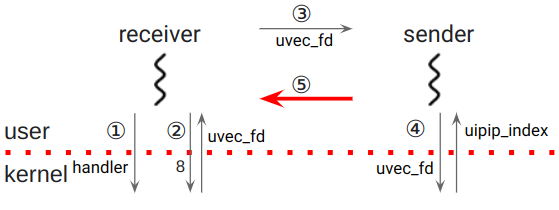
\includegraphics[width=\textwidth]{uintrInit}
  \caption{Phase d'initialisation des \uintr{}}
  \label{fig:initUintr}
\end{figure}

Maintenant que nous avons vu l'initialisation, nous allons pouvoir voir comment l'envoi d'interruption est réalisé, comme illustré dans la figure \ref{fig:sendUintr} :

\begin{enumerate}[label=\protect\circled{\arabic*}]
  \item L'émetteur utilise l'instruction \code{senduipi} avec l'indice récupéré lors de l'initialisation.
  L'unité de calcul peut accéder au tableau \emph{UITT} qui se trouve dans le registre \code{IA32_UINTR_TT}.
  Elle peut vérifie que l'indice se trouve bien dans le tableau, en utilisant la taille qui se trouve dans le registre \code{IA32_UINTR_MISC}.
  De plus, il s'assure que l'entrée dans le \emph{UITT} est valide.
  À partir de l'indice donné à l'instruction, l'émetteur peut récupérer l'adresse de l'\emph{UPID} et le vecteur \uintr{} à envoyer au récepteur.
  Dans la zone mémoire de l'\emph{UPID}, il écrit le vecteur \uintr{} à envoyer et détermine s'il faut également envoyer une interruption ordinaire.
  En effet, les interruptions en espace utilisateur utilisent les interruptions ordinaires,
  et l'envoi de celles-ci dépend de si une interruption ordinaire n'a pas déjà été envoyée.
  Dans notre cas, nous considérons que c'est le premier envoi.
  \item Donc, l'émetteur va récupérer le vecteur d'interruption ordinaire dans le registre \code{IA32_UINTR_MISC} et
  sélectionner le registre \emph{ICR} correspondant au vecteur "ordinaire".
  Ensuite, il va récupérer l'\emph{APIC ID} dans l'\emph{UPID} et l'écrire dans le registre \emph{ICR}.
  Cela permettra d'envoyer l'interruption ordinaire à l'unité de calcul correspondante.
  \item L'\emph{APIC} va recevoir l'interruption, puis elle va comparer le vecteur d'interruption ordinaire reçu avec celui qui se trouve dans l'\emph{UPID}, qu'il connaît grâce au registre \code{IA32_UINTR_PD}.
  Si les vecteurs sont identiques, l'\emph{APIC} va pouvoir déclencher le système de traitement des \uintr{}, sinon, elle va utiliser le mécanisme habituel des \emph{IRQ}.

  \item Le système de traitement des \uintr{} va donc indiquer dans l'\emph{UPID} que l'interruption ordinaire a déjà été envoyée,
  puis va commencer le déclenchement des handlers pour tous les vecteurs \uintr{} reçus, en partant du plus grand, 63, jusqu'au plus petit, 0.
  \code{IA32_UINTR_RR} est utilisé à cette étape.
  Dans notre exemple, nous en avons un seul qui est 8.
  L'\emph{APIC} va donc ordonner à l'unité de calcul de changer de pile si une pile alternative est disponible dans
  le registre \code{IA32_UINTR_STACKADJUST}, empiler les registres nécessaires, empiler le vecteur \uintr{} (donc 8 dans l'exemple) et aller à l'adresse du handler qui est disponible dans le registre \code{IA32_UINTR_HANDLER}.
\end{enumerate}

\begin{figure}[H]
  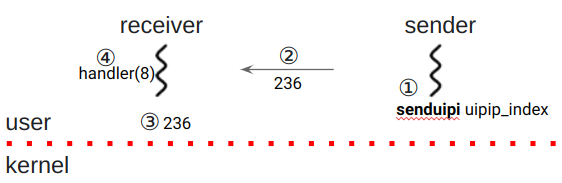
\includegraphics[width=\textwidth]{uintrSend}
  \caption{L'envoi d'une \uintr{}}
  \label{fig:sendUintr}
\end{figure}

Le mécanisme habituel des \emph{IRQ} peut être utilisé dans le cas où l'\uintr{} est déclenchée depuis le noyau et
dans le cas où le thread destinataire n'est pas ordonnancé ou est dans un appel système interruptible.

\subsubsection{Partage du descripteur de fichier}
\label{sec:shareFD}

Pour partager le descripteur de fichier, il y a plusieurs façons possibles.

Dans nos tests du mécanisme entre processus, nous avons utilisé l'héritage des descripteurs de fichier.
Dans nos tests du mécanisme entre threads, nous avons utilisé un appel système qui permet d'enregistrer tous les threads du processus comme émetteurs, sans utiliser le descripteur de fichier, % \verb|uintr_register_self()|
mais il est possible d'utiliser une variable globale pour y mettre le descripteur de fichier.

Dans le cas où les deux processus sont indépendants, on peut utiliser l'appel système \code{pidfd_getfd} qui permet de dupliquer le descripteur de fichier d'un autre processus s'il a le même propriétaire et si l'on connaît son \emph{PID} et le numéro du descripteur de fichier.
Nous avons donc testé en partageant le numéro de descripteur de fichier avec un pipe.
On aurait aussi pu passer par un fichier ou par des sockets.

Par la suite, dans \emph{NewMadeleine}, nous avons utilisé le système d'URL à la connexion qui permet l'envoi de paramètres.
Donc nous avons ajouté un paramètre avec la valeur du descripteur de fichier.

\subsection{Tests du mécanisme}

Nous avons donc effectué des tests du mécanisme avec des exemples minimaux de communication entre processus.
Nous examinerons les plus pertinents dans cette section.

Tout d'abord, des tests pour mesurer le temps d'envoi d'interruption en espace utilisateur entre deux threads et deux processus.

Pour le test d'envoi entre deux threads, il commence par créer un nouveau thread qui va commencer par se "bind" à une unité de calcul.
Nous le verrons en détail dans la section \ref{sec:latencyMesure}.

Il va ensuite enregistrer un handler d'interruption, démasquer les interruptions, enregistrer tous les threads du processus comme émetteurs avec l'appel système \code{uipi_index <- uintr_register_self(vector)},\\
(uipi_index est global au processus) et attendre grâce à une boucle.

Pendant ce temps-là, le thread principal attend une seconde.
Ce temps est arbitraire et laisse le temps au thread d'enregistrer un handler d'interruption.
Après son attente, il va se "bind" à une unité de calcul puis envoyer une interruption.
Pour cela, nous commençons par enregistrer le temps processeur actuel, puis nous utilisons l'instruction \code{senduipi} avec la variable globale \code{uipi_index}.
Une fois que le handler d'interruption se déclenche, on enregistre le temps actuel du processeur pour ensuite calculer la différence.
Ce test est capable de faire cette mesure plusieurs fois.
Il finit par imprimer les différences de temps dans la console et par désallouer et de-enregistrer les \uintr{} et les autres structures.

Pour le teste d'envoi entre deux processus, il commence par créer un pipe pour l'envoi du descripteur de fichier et une zone de mémoire partagée pour stocker les mesures de temps.
Puis le processus se fork en deux, le premier devient l'émetteur et le second le récepteur.
Comme pour la version avec threads, ils se "bind" à une unité de calcul.
Le récepteur enregistre un handler d'interruption et récupère un descripteur de fichier avec l'appel système \code{uvec_fd <- uintr_vector_fd(vector)} qu'il envoie dans le pipe avant d'attendre grâce à une boucle.
L'émetteur reçoit le numéro du descripteur de fichier, il connaît déjà le \emph{PID} du processus grâce au fork,
il peut donc utiliser \code{pidfd_getfd} pour dupliquer le descripteur de fichier.
Avec ce descripteur, il s'enregistre en tant qu'émetteur d'\uintr{}.
La mesure du temps et l'envoi d'interruption fonctionnent de la même manière que pour la version avec threads.
On peut aussi effectuer la mesure plusieurs fois et on imprime et termine proprement.

On verra les résultats de ces mesures dans la section \ref{sec:performance}.

Un test où le thread s'auto-interrompt tout simplement en faisant un \code{uipi_index <- uintr_register_self(vector)},\\
puis un \code{senduipi uipi_index}, et on fait la mesure de la même façon que pour les autres tests.

Pour les tests avec la pile alternative, nous avons un test très simple qui est basé sur celui qui s'auto-interrompt, et nous modifions les tests d'envoi entre deux processus ou threads pour mesurer l'impact les performances.
Il est bien sûr possible d'activer ou non l'utilisation de la pile alternative.
Pour définir cette nouvelle pile, on le fait juste après avoir enregistré le handler d'interruption et avant le démasquage.

Un test de démasquage des \uintr{} dans un handler d'interruption.
Il nous permet de voir que c'est tous à fait possible et cela pose des problématiques similaires à celles des signaux.

Un test consiste à envoyer plusieurs interruptions d'affilée.
Il nous permet de voir qu'il y a une différence de comportement par rapport aux signaux.
Quand on reçoit une interruption et que le handler d'interruption est déclenché, le comportement est le même,
c'est-à-dire que les interruptions vont s'écraser et le handler d'interruption se déclenchera à nouveau une fois.
La différence réside dans le fait que si l'on effectue plusieurs interruptions avant que le handler d'interruption ne se déclenche,
les interruptions s'écrasent également à ce moment-là.
Ainsi, le handler d'interruption ne se déclenchera qu'une seule fois lorsque l'on effectue deux interruptions successives.
Avec les signaux, en revanche, le handler de signal se déclencherait deux fois pour deux émissions de signal successives car le handler est déjà déclenché dès le premier signal.

Grâce à un test, nous avons constaté qu'actuellement on peut enregistrer plusieurs fois le même descripteur de fichier,
ce qui mène à des doublons dans le tableau \emph{UITT} avec plusieurs \emph{UITTE} pour le même couple vecteur / \emph{UPID}.
Cette limitation de l'implémentation noyau est documentée dans le patch et accompagnée d'un commentaire \emph{TODO}.

\subsection{Correction d'un bug dans le patch noyau}

En manipulant le mécanisme, nous sommes tombés sur un bug qui concerne l'utilisation d'une pile alternative.
Comme pour les signaux, il est possible de définir une pile alternative.
Cette nouvelle pile est utilisée au moment où le handler est déclenché.
L'interface pour définir la pile alternative est la même pour les signaux et les \uintr{}.
Dans les manuels (des signaux et des \uintr{}), il est bien indiqué que l'utilisateur doit lui-même allouer une zone mémoire consacrée à la nouvelle pile,
et il a également la responsabilité de libérer la mémoire une fois le handler dé-enregistré.
Il est bien indiqué que l'utilisateur doit donner l'adresse de début (\emph{base address}) de la zone mémoire,
ainsi que la taille, à l'appel système qui définit la pile alternative.
Pour les \uintr{}, l'appel système est \code{uintr_alt_stack(spAddress, size)}.
Il faut noter qu'une pile empile les éléments vers le haut, c'est-à-dire que l'adresse du pointeur de pile décroît à l'ajout d'un élément.
Donc, pour utiliser la zone mémoire dédiée à la pile, il faut partir de la fin.
Du côté du noyau, le mécanisme des signaux garde en mémoire l'adresse et la taille de la pile pour le moment où le handler doit être déclenché.
Le calcul du pointeur de pile de la nouvelle pile se fait donc juste avant de déclencher le handler.
Pour les \uintr{}, le noyau se contente juste d'enregistrer l'adresse dans le registre dédié \code{IA32_UINTR_STACKADJUST},
et le processeur utilise l'adresse telle quelle comme pointeur de pile.
On est donc confronté à un bug de débordement mémoire car on part du début de la zone mémoire.
Il y a bien un test dans le patch du noyau qui vérifie ce cas, mais mal.
Nous sommes tombés sur ce bug au moment d'utiliser les \uintr{} dans \emph{NewMadeleine},
qui manipule bien plus la mémoire qu'un simple test.
Nous nous sommes retrouvés avec des problèmes de corruption mémoire, des défauts de segmentation et des "double free detected".
Nous avons donc corrigé le test du patch du noyau ainsi que l'appel système.
Pour ce faire, on ajoute la taille de la zone mémoire à l'adresse avant de l'écrire dans le registre \code{IA32_UINTR_STACKADJUST}.
Nous avons donc effectué une \emph{Pull request} \cite{pullRequestAltStackFix} sur le dépôt GitHub du patch,
et à l'heure où nous écrivons ce document, il n'a toujours pas été appliqué par \intel{}.

\subsection{Mesure de la latence}
\label{sec:latencyMesure}

Pour mesurer la latence entre le moment où on envoie une interruption et où l'interruption est reçue par le handler,
on fait deux mesures de temps.
Pour faire les mesures de temps, on utilise \code{clock_gettime} qui utilise l'instruction \code{rdtsc} et retourne le temps actuel du processeur.
On fait une première mesure juste avant d'envoyer une interruption et une seconde au tout début du handler.
Pour obtenir la latence, on a juste à soustraire la première mesure à la seconde.

Nous avons regardé le code assembleur pour nous assurer de la mesure.
Pour l'envoi, que l'on peut voir en listing \ref{lst:sendUintrAsm}, on peut constater qu'entre la mesure et l'instruction d'envoi,
il y a seulement une lecture mémoire qui n'est pas très coûteuse.
Du côté de la réception, que l'on peut voir en listing \ref{lst:handlerUintrAsm},
on voit la sauvegarde des registres généraux au début du handler.
Cette sauvegarde ajoute un petit surcoût, mais il est obligatoire.
Le compilateur \emph{GCC} nous force à mettre le flag \code{general-regs-only} pour compiler un handler d'interruption et donc sauvegarder les registres généraux.
On peut voir la déclaration d'un handler avec la mesure du temps en listing \ref{lst:unitrHandler}.

\begin{lstlisting}[language={[x86masm]Assembler}, caption=Code assembleur de l'envoi d'\uintr{}, label={lst:sendUintrAsm}]
	call	clock_gettime@PLT
	movq	uipi_index(%rip), %rax
	senduipi	%rax
\end{lstlisting}

% \begin{figure}[H]
%   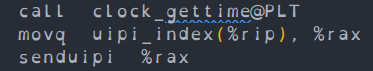
\includegraphics[width=\textwidth]{senduipiTimeThreadO3}
%   \caption{Code assembleur de l'envoi d'\uintr{}}
%   \label{fig:sendUintrAsm}
% \end{figure}

\begin{lstlisting}[language={[x86masm]Assembler}, caption=Code assembleur de l'handler \uintr{}, label={lst:handlerUintrAsm}]
  handler:
  .LFB203:
    .cfi_startproc
    .cfi_def_cfa_offset 16
    pushq	%r11
    .cfi_def_cfa_offset 24
    .cfi_offset 11, -24
    pushq	%r10
    .cfi_def_cfa_offset 32
    .cfi_offset 10, -32
    pushq	%r9
    .cfi_def_cfa_offset 40
    .cfi_offset 9, -40
    pushq	%r8
    .cfi_def_cfa_offset 48
    .cfi_offset 8, -48
    pushq	%rdi
    .cfi_def_cfa_offset 56
    .cfi_offset 5, -56
    movl	$1, %edi
    pushq	%rsi
    .cfi_def_cfa_offset 64
    .cfi_offset 4, -64
    leaq	ts2(%rip), %rsi
    pushq	%rcx
    .cfi_def_cfa_offset 72
    .cfi_offset 2, -72
    pushq	%rdx
    .cfi_def_cfa_offset 80
    .cfi_offset 1, -80
    pushq	%rax
    .cfi_def_cfa_offset 88
    .cfi_offset 0, -88
    subq	$8, %rsp
    .cfi_def_cfa_offset 96
    cld
    call	clock_gettime@PLT
\end{lstlisting}

% \begin{figure}[H]
%   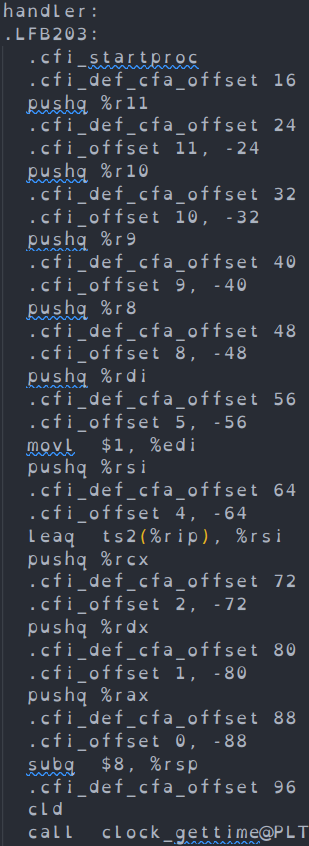
\includegraphics[height=\textwidth]{handlerTimeThreadO3}
%   \caption{Code assembleur de l'handler \uintr{}}
%   \label{fig:handlerUintrAsm}
% \end{figure}

\begin{lstlisting}[language=c, caption=Déclaration du handler \uintr{}, label={lst:unitrHandler}]
  __attribute__((target("general-regs-only")))
  __attribute__((interrupt))
  void handler(struct __uintr_frame* ui_frame, u64 vector) {
    clock_gettime(CLOCK_MONOTONIC, &ts2);
\end{lstlisting}

% \begin{figure}[H]
%   \centering
%   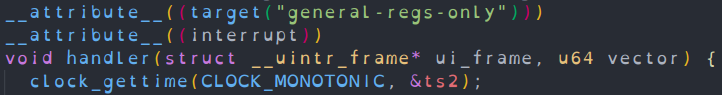
\includegraphics[width=\textwidth]{handlerDeclaration}
%   \caption{Déclaration du handler \uintr{}}
%   \label{fig:unitrHandler}
% \end{figure}

Nous faisons la mesure de la même façon pour les signaux.

Pour ne pas perturber la mesure, il faut "bind" les threads à une unité de calcul.
"bind" consiste à demander au noyau de toujours ordonnancer le thread sur la même unité de calcul.
Pour ce faire nous utilisons la bibliothèque \emph{hwloc} \cite{hwloc}.
Il est donc important de "bind" les threads pendant les mesures car dans le cas contraire,
le noyau va changer le thread d'unité de calcul, ce qui va amener à un surcoût non négligeable.
En effet, le changement d'unité est un peu coûteux et invalide certains caches.
"bind" les threads nous permet aussi de contrôler le placement de ceux-ci, c'est-à-dire si on met le thread émetteur et le thread récepteur sur deux unités de calcul proches ou distantes.
Comme nous le verrons dans la section \ref{sec:performance}, le placement a un impact sur la latence des \uintr{}.

Il est aussi important de fixer la fréquence de tous les core du CPU pour avoir des mesures reproductibles.

\subsection{Performances}
\label{sec:performance}

Dans cette section, nous allons voir des mesures de la latence des \uintr{} dans différents contextes.
La fréquence des unités de calcul est fixée à 2 GHz lors des mesures.
Les mesures faites avec le turbo boost activé montent à 3.8 GHz.
Les mesures de latence sont en nanosecondes.
Il est intéressant de noter que sur une unité de calcul cadencée à une fréquence de 2 GHz, elle exécute environ deux instructions par nanoseconde. % plus 2 cycle
Certaines mesures, que ce soit avec les \uintr{} ou les signaux, sont très élevées mais sont très peu nombreuses.
Elles sont certainement liées au système.
Dans les graphiques, nous avons donc coupé les valeurs qui dépassent les 8000 nanosecondes. % on considère juste les valeurs entre 0 et 8000 ns
Nous avons défini trois placements à partir de la topologie de la machine fournie par \atos{}.
Vous pouvez trouver la topologie de la machine sur la figure \ref{fig:lstopo}.

Les trois placements sont les suivants :
\begin{itemize}
  \item Le placement "proche" consiste à placer les threads sur deux unités de calcul proches mais pas dans le même core.
  \item Le placement "éloigné" consiste à placer les threads sur deux unités de calcul qui sont dans le même CPU et qui sont éloignées.
  \item Le placement "très éloigné" consiste à placer les threads sur deux unités de calcul qui se trouvent sur deux CPU différents.
\end{itemize}

Les mesures que nous allons présenter ont été faites sans que la pile alternative ne soit activée.
Nous avons bien fait des mesures avec la pile alternative des \uintr{} activée et nous n'avons vu aucune différence,
car l'utilisation de cette pile amène seulement à une copie de la mémoire d'un registre à un autre si le registre contient une adresse, ce qui est très peu coûteux.

Dans nos graphiques, nous appelons une mesure une itération.
Nous faisons donc un million d'itérations et nous n'affichons pas la première, car cette itération est énormément perturbée notamment par le coût de chargement des caches.

Dans les graphiques, nous avons représenté la mesure de la latence par des points bleus pour les signaux et par des points rouges pour les \uintr{}.
Nous ne cherchons pas à expliquer les mesures des signaux, elles sont juste là pour comparer les \uintr{} avec un mécanisme qui passe par le noyau.

Sur le graphique \ref{subfig:latency1e6ThreadsNT}, les itérations sont représentées sur l'axe des abscisses et la latence sur l'axe des ordonnées.
Bien sûr, plus la latence est basse, mieux c'est.
Nous observons que le mécanisme a une latence d'environ 642 nanosecondes, ce qui est environ 4.75 fois plus rapide que les signaux.

On voit qu'il y a deux groupes de mesures :
\begin{itemize}
  \item Un autour des 642 nanosecondes qui comporte la majorité des mesures.
  On le voit bien dans le tableau \ref{tab:latency1e6ThreadsNT} qui se trouve juste en dessous du graphique.
  En effet, entre la mesure minimum et la mesure à 95\%, il y a une différence de 19 nanosecondes.
  On peut voir cette distribution aussi dans l'histogramme sur la figure \ref{fig:distribution}.
  Cet histogramme porte sur des plages de 300 nanosecondes.
  On voit bien pour les \uintr{}, en orange, que la majorité se trouve sur la bande entre 300 et 600 nanosecondes.
  \item Un autre autour de 2700 nanosecondes qui correspond certainement au moment où l'interruption n'a pas pu être reçue car le thread était dans le noyau.
\end{itemize}

Pour un mécanisme qui fonctionne au niveau des instructions, on pourrait s'attendre à une latence moins grande,
mais le mécanisme est bien plus rapide que le fait de passer par le système.
% il serai intéressant de comparer avec la latence d'une IRQ 236 et non uintr
% TODO: ce qu'on en pense, c'est bon ?

\begin{figure}[H]
  \begin{subfigure}{\textwidth}
    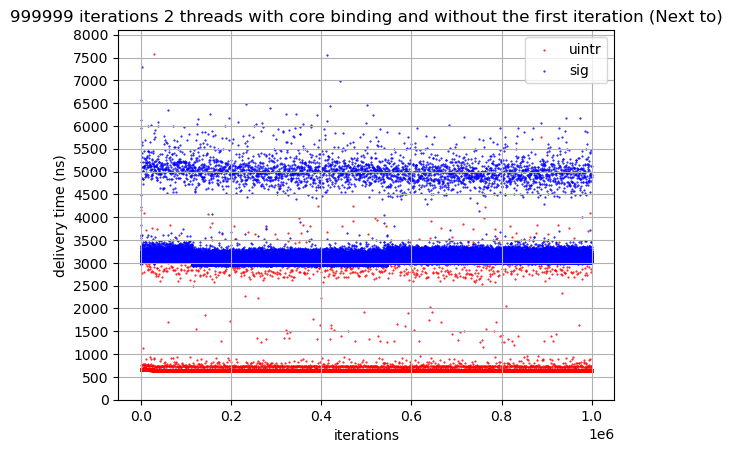
\includegraphics[width=\textwidth]{latency/1e6ThreadsNT}
    \caption{}
    \label{subfig:latency1e6ThreadsNT}
  \end{subfigure}
  \begin{subtable}{\textwidth}
    \centering
    \begin{tabular}{| l | l | l | l | l | l | l | l |}
      \hline
      &\bf mean &\bf std &\bf min  &\bf 10\% &\bf 50\% &\bf 95\% &\bf max\\
      \hline
      \bf sig   & 3065 & 160 & 2920 & 3001 & 3054 & 3157 & 68532\\
      \hline
      \bf uintr & 643  & 90  & 629  & 638  & 642  & 648  & 65973\\
      \hline
    \end{tabular}
    \caption{}
    \label{tab:latency1e6ThreadsNT}
  \end{subtable}
  \caption{Mesures de latence entre deux threads avec un placement proche}
  \label{fig:latency1e6ThreadsNT}
\end{figure}

\begin{figure}[H]
  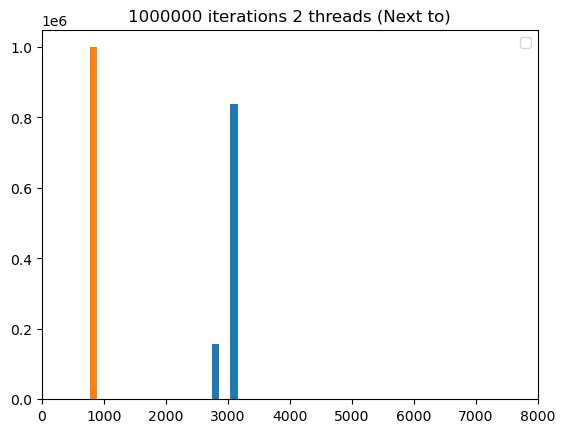
\includegraphics[width=\textwidth]{latency/distribution}
  \caption{Histogramme de distribution des mesures de la latence entre deux threads avec un placement proche}
  \label{fig:distribution}
\end{figure}

Nous avons fait les mêmes mesures entre deux processus et les valeurs sont très similaires, peu importe le placement,
car le mécanisme fonctionne au niveau des threads.
On peut retrouver ces mesures en annexe sur la figure \ref{fig:latency1e6ProcessNT}.

En comparant les mesures de latences entre le placement proche et éloigné on voit une petite différence de 10 nanosecondes de plus,
on peut voir ça sur la figure \ref{fig:latency1e6ThreadsF}.

Quand on compare entre le placement proche et très éloigné on voit une grande différence qui est due notamment au fait de passer d'un noeud mémoire NUMA à un autre.
On a donc une différence d'environ 172 nanosecondes de plus.
Le graphique nous montre également une plus grande dispersion de la latence avec la majorité qui est toujours en-dessous de 1000 nanosecondes.
On retrouve ces mesures sur la figure \ref{fig:latency1e6ThreadsVF} juste en-dessous.
\begin{figure}[H]
  \begin{subfigure}{\textwidth}
    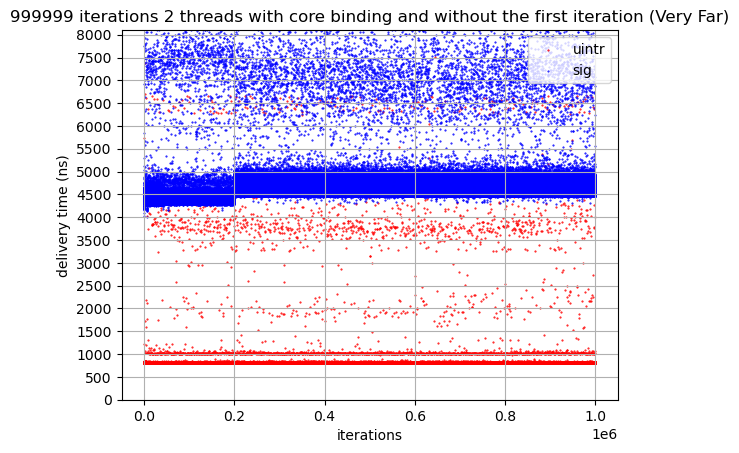
\includegraphics[width=\textwidth]{latency/1e6ThreadsVF}
    \caption{}
    \label{subfig:latency1e6ThreadsVF}
  \end{subfigure}
  \begin{subtable}{\textwidth}
    \centering
    \begin{tabular}{| l | l | l | l | l | l | l | l |}
      \hline
      &\bf mean &\bf std &\bf min  &\bf 10\% &\bf 50\% &\bf 95\% &\bf max\\
      \hline
      \bf sig   & 4601 & 403 & 4009 & 4396 & 4561 & 4796 & 58200\\
      \hline
      \bf uintr & 818  & 136 & 801  & 810  & 814  & 820  & 58072\\
      \hline
    \end{tabular}
    \caption{}
    \label{tab:latency1e6ThreadsVF}
  \end{subtable}
  \caption{Mesures de latence entre deux threads avec un placement très éloigné}
  \label{fig:latency1e6ThreadsVF}
\end{figure}

Quand on augmente la fréquence des unités de calcul la latence diminue.
Pour se faire on active le turbo boost du CPU.
On le voit sur les mesures de la figure \ref{fig:latency1e6ThreadsNT-TB} pour le placement proche mais c'est également le cas pour le placement éloigné et le très éloigné en figure \ref{fig:latency1e6ThreadsF-TB} et figure \ref{fig:latency1e6ThreadsVF-TB}.

\begin{figure}[H]
  \begin{subfigure}{\textwidth}
    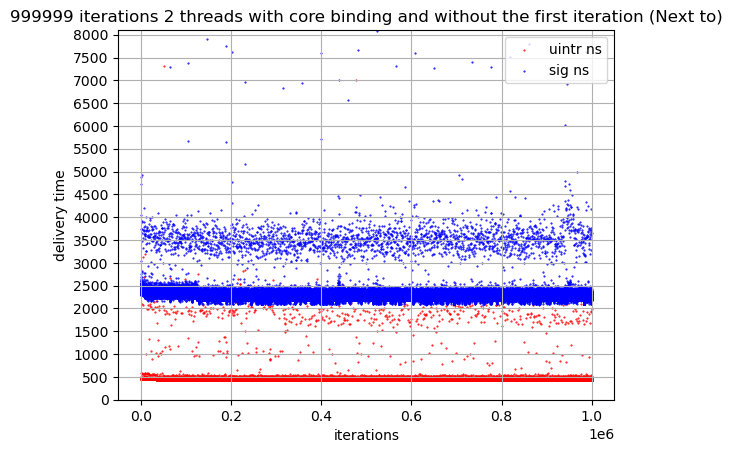
\includegraphics[width=\textwidth]{latency/1e6ThreadsNT+TB}
    \caption{}
    \label{subfig:latency1e6ThreadsNT-TB}
  \end{subfigure}
  \begin{subtable}{\textwidth}
    \centering
    \begin{tabular}{| l | l | l | l | l | l | l | l |}
      \hline
      &\bf mean &\bf std &\bf min  &\bf 10\% &\bf 50\% &\bf 95\% &\bf max\\
      \hline
      \bf sig   & 2262 & 294 & 2081 & 2216 & 2251 & 2357 & 283171\\
      \hline
      \bf uintr & 442  & 313 & 426  & 437  & 440  & 450  & 311486\\
      \hline
    \end{tabular}
    \caption{}
    \label{tab:latency1e6ThreadsNT-TB}
  \end{subtable}
  \caption{Mesures de latence entre deux threads avec un placement proche et le turbo boost activé}
  \label{fig:latency1e6ThreadsNT-TB}
\end{figure}

Nous n'avons fait aucune mesure de latence pour les threads bloqués et interruptibles.
